% Journal of Computer Applications in Archaeology (JCAA) — Revision v0.2  (R&R of #280)
% Ubiquity Press — Harvard (natbib) citation style, blind review
%
% ============================================================================
% STATUS OF THIS FILE — read before compiling / reading
% ============================================================================
% This is the v0.2 PROSE draft (revision step #1 in HANDOFF_20260803.md §6).
% The central claim of v0.1 is WITHDRAWN and REPLACED: the reported AUC ladder
% is an evaluation artefact, not a bias-correction gain. Every numbered sentence
% is sourced to review_package_20260727/10_SET_KLAIM_TERKOREKSI.md (the
% authoritative claim set). DO NOT draft further from 08_HANDOFF_BABAK2.md §3 —
% three of its five claims are withdrawn (K5/K6/K7).
%
% OPEN ITEMS BEFORE THIS CAN BE SUBMITTED (handoff §6 steps 2–6, then PI):
%   [TITLE]   v0.2 title is candidate 3 ("evaluation incomparability" framing).
%             Claim-set §4 + response-plan §3 vet candidates 1 & 3 as safe;
%             candidate 3 used here. PI DECISION (item E) — confirm or swap to 1.
%   [FIGURES] Figures marked with \figtodo{...} do NOT yet exist (revision
%             blocks E & F, step #2). \figtodo renders a placeholder box so this
%             file COMPILES NOW; replace each with \includegraphics once built.
%             Existing figures (fig1...fig13) keep their current filenames.
%   [CITES]   A few ENM citations the response letter promises could not be
%             verified against a source and are marked [NEEDS CITATION: ...]
%             inline rather than fabricated. Resolve before submission.
%   [SIG]     verify_headline_numbers.py must be re-run; re-run full SIG sign-off
%             (step #6). v0.2 currently exists only as this draft, so G2/G8/G9
%             are not yet runnable — they gate on exactly this prose.
% ============================================================================

\documentclass[12pt]{article}
\usepackage[utf8]{inputenc}
\usepackage[a4paper, margin=2.5cm]{geometry}
\usepackage{setspace}
\usepackage{graphicx}
\graphicspath{ {./figures/} }
\usepackage{amsmath}
\usepackage{amssymb} % for \checkmark (used as \cmark in Table 2)
\usepackage{booktabs}
\usepackage{array}
\usepackage{xcolor}
\newcommand{\cmark}{\checkmark}
\usepackage{url}
\usepackage{hyperref}
\usepackage{lineno}
\linenumbers

% Harvard citation style (author-year) via natbib
\usepackage[round]{natbib}
\bibliographystyle{plainnat}

% Double spacing for review
\doublespacing

% Placeholder for figures not yet built (revision blocks E & F).
% Renders a labelled box so the file compiles cleanly; swap for
% \includegraphics once the figure exists.
\newcommand{\figtodo}[1]{%
  \begin{center}%
  \fbox{\parbox[c][3.6cm][c]{0.86\textwidth}{\centering\textit{[Figure pending --- revision blocks E/F: #1]}}}%
  \end{center}}

% [TITLE] PI decision (item E). Candidate 3; rests on evaluation incomparability.
\title{An Evaluation Artefact in Presence--Background Archaeological Modelling:\\
Evidence from East Java and a Corrected Comparison Protocol}

\author{Mukhlis Amien\textsuperscript{1,*}, Go Frendi Gunawan\textsuperscript{1}}

\date{%
\textsuperscript{1}Lab Data Sains, Universitas Bhinneka Nusantara, Indonesia\\
\textsuperscript{*}Corresponding author: amien@ubhinus.ac.id%
}

\begin{document}

\maketitle

\begin{abstract}
\noindent
Presence--background (presence-only) archaeological predictive models are usually evaluated by cross-validation against the same background points used to fit them.
We show that this practice can manufacture an apparent performance gain where none exists, and that the artefact is hard to see because it is produced by exactly the step a researcher takes to be rigorous.
We built a settlement suitability model for East Java (378 presences; XGBoost, RandomForest and a maxnet-equivalent Maximum Entropy model under fixed spatial-block cross-validation) and originally reported a monotone AUC ladder, $0.659 \rightarrow 0.751$ (seed-averaged; best run $0.768$), which we attributed to increasingly realistic pseudo-absence (background) design.
A benchmark requested by a reviewer refuted that attribution.
When each background design is scored against a common evaluation background held fixed across designs, redesigning the background contributes \textbf{$-0.014$ AUC} averaged over three algorithms, whereas adding a single hydrological feature contributes \textbf{$+0.042$ AUC} (positive in 12/12 paired comparisons).
The reported gain is an artefact of evaluation: each design was scored against the negatives it had selected for itself, and the resulting inflation is positive in 60/60 seed$\times$algorithm cells (mean $+0.037$).
We establish the mechanism with four synthetic worlds of known ground truth: the selection criterion computed on a design's own background has \emph{no interior optimum}---its maximum always sits at the edge of whatever dial is swept---and reported and true performance move in opposite directions on the real data.
Equivalence confidence intervals reject the published ladder gain in 12/12 algorithm$\times$evaluation-background cells.
We withdraw the taphonomic interpretation we had built on the ladder, correct two defects in our own diagnostics (an incomplete volcano inventory and a correlation that does not reproduce across seeds), and propose a corrected protocol: compare background designs only on a held-fixed evaluation background, declare the evaluation availability domain of every metric, and seed-ensemble priority maps ($k \geq 7$), which a single seed is too unstable to support.
The contribution is the diagnosis and the protocol, not a new site-prediction claim.
\end{abstract}

\noindent\textbf{Keywords:} presence-background modelling; pseudo-absence design; evaluation artefact; target-group background; spatial cross-validation; survey bias; East Java

% ============================================================================
\section{Introduction}
% ============================================================================

Predictive settlement modelling in Java is difficult because the observed archaeological record is shaped as much by preservation and discovery as by past settlement behaviour.
Known site maps are incomplete and strongly conditioned by survey history; active volcanism and tephra deposition can bury older surfaces; and from a computational standpoint the combination produces label noise in pseudo-absence design and inflates validation when spatial dependence is mishandled.
This paper addresses a narrower question than it first appears to: \emph{how do you know that redesigning the background points improved a presence--background model?}
The answer we offer is uncomfortable, because it is the answer we had to give about our own model.

\subsection{What presence--background models are, and why their evaluation is delicate}

Presence--background (presence-only) models learn a suitability surface from known presences and a set of background points that stand in for the available environment.
They are the workhorse of ecological niche modelling (ENM) and species distribution modelling (SDM) \citep{elith2006, phillips2006} and of much archaeological predictive modelling \citep{verhagen2012, kvamme2006}.
They are acutely sensitive to sample-selection bias, especially when the background does not reflect the same observation process as the presences \citep{phillips2009, araujo2006, wisz2009, lobo2010}.
The standard correction for survey-biased data is target-group background (TGB): draw background points from the area a survey could plausibly have reached, so that the model learns presence against a realistic ``available'' set rather than against the whole landscape \citep{phillips2009}.

A model improved in this way is judged by cross-validation against held-out points, and the held-out \emph{negatives} are drawn from the same background distribution the model was trained on.
This is where the delicacy lies.
If two background designs are each scored against their own background, the comparison is not identified: a design that makes its own background easier to separate from presences will look better, for a reason that has nothing to do with how well either model captures the phenomenon.
Random train/test splits are known to overestimate transfer under spatial clustering \citep{kohavi1995}; spatially structured cross-validation is the recommended corrective \citep{roberts2017, valavi2019}.
But spatial blocking fixes where the folds are; it does not, by itself, fix \emph{which} background the held-out negatives come from.
That second choice is the subject of this paper.

\subsection{Four reasons a site may be absent, and which one we model}

\label{sec:taxonomy}

Following a reviewer's taxonomy, a site may be absent from the record for four distinct reasons, and conflating them is the central interpretive hazard of this literature:

\begin{enumerate}
  \item \textbf{Environmentally unsuitable} --- the location was never attractive for settlement.
  \item \textbf{Not surveyed} --- a site could be there, but no one has looked there.
  \item \textbf{Buried} --- a site was there and is now below the detectable surface.
  \item \textbf{Destroyed} --- a site was there and has since been erased.
\end{enumerate}

\textbf{This paper models suitability only} (mechanism 1).
The other three are the interpretive frame, not the output of the model.
A low suitability score does not distinguish ``never settled'' from ``buried'' or ``destroyed''; a high suitability score does not assert that a site exists.
We state this restraint up front because the earlier version of this manuscript overreached it, and the retraction of that overreach is reported in \S4.

\subsection{Contribution and relation to prior work}

This is the first revise-and-resubmit the project has received, and the reviewer who asked us to benchmark against Maximum Entropy \citep[R1-D;][]{elith2006} asked for what turned out to be the decisive analysis.
The benchmark refuted our own central claim (\S3.2): the AUC ladder we attributed to background realism is an evaluation artefact.
We have therefore not revised the paper's argument; we have replaced it.
The same empirical material now supports a narrower and, we believe, more useful proposition: \emph{background designs in presence--background modelling cannot be compared unless the evaluation background is held fixed, and a selection criterion computed on a design's own background has no interior optimum.}

Our contribution sits \emph{inside} the ENM literature rather than beside it.
The target-group background correction is a known technique \citep{phillips2009}, and the concern that background choice drives reported performance is not new in ecology \citep{barbet2012, senay2013, georganos2021}.
Recent machine-learning work in archaeology shows strong performance gains when spatial context and terrain logic are integrated, while flagging data-quality and validation constraints \citep{castiello2021, wang2023, comer2023}.
\textbf{[NEEDS CITATION: Yaworsky et al.\ 2020; Banks et al.\ (ecocultural niche modelling); Franklin, \emph{Mapping Species Distribution}; Howey; Noviello et al. --- add verified entries before submission.]}
What we add is not ``background design matters'' but a quantification of \emph{why} it appears to matter when it does not: the comparison becomes a tautology of the evaluation set, and the resulting inflation is of the same order as the gain typically reported.

The honest shape of this revision is worth stating.
A title can be softened to match weaker evidence, but when the evidence supports a different proposition, softening is not enough; the proposition has to be replaced.
Retitling from a bias-correction claim to an evaluation-artefact finding is that kind of replacement, and we believe it is what the reviewer's request required.

\subsection{Study area}

The study area is province-scale East Java (approximate bounds 111--115$^\circ$E, 9--6.5$^\circ$S), processed in EPSG:32749.
Figure~\ref{fig:studyarea} locates the area and the presences.

\begin{figure}[h]
\centering
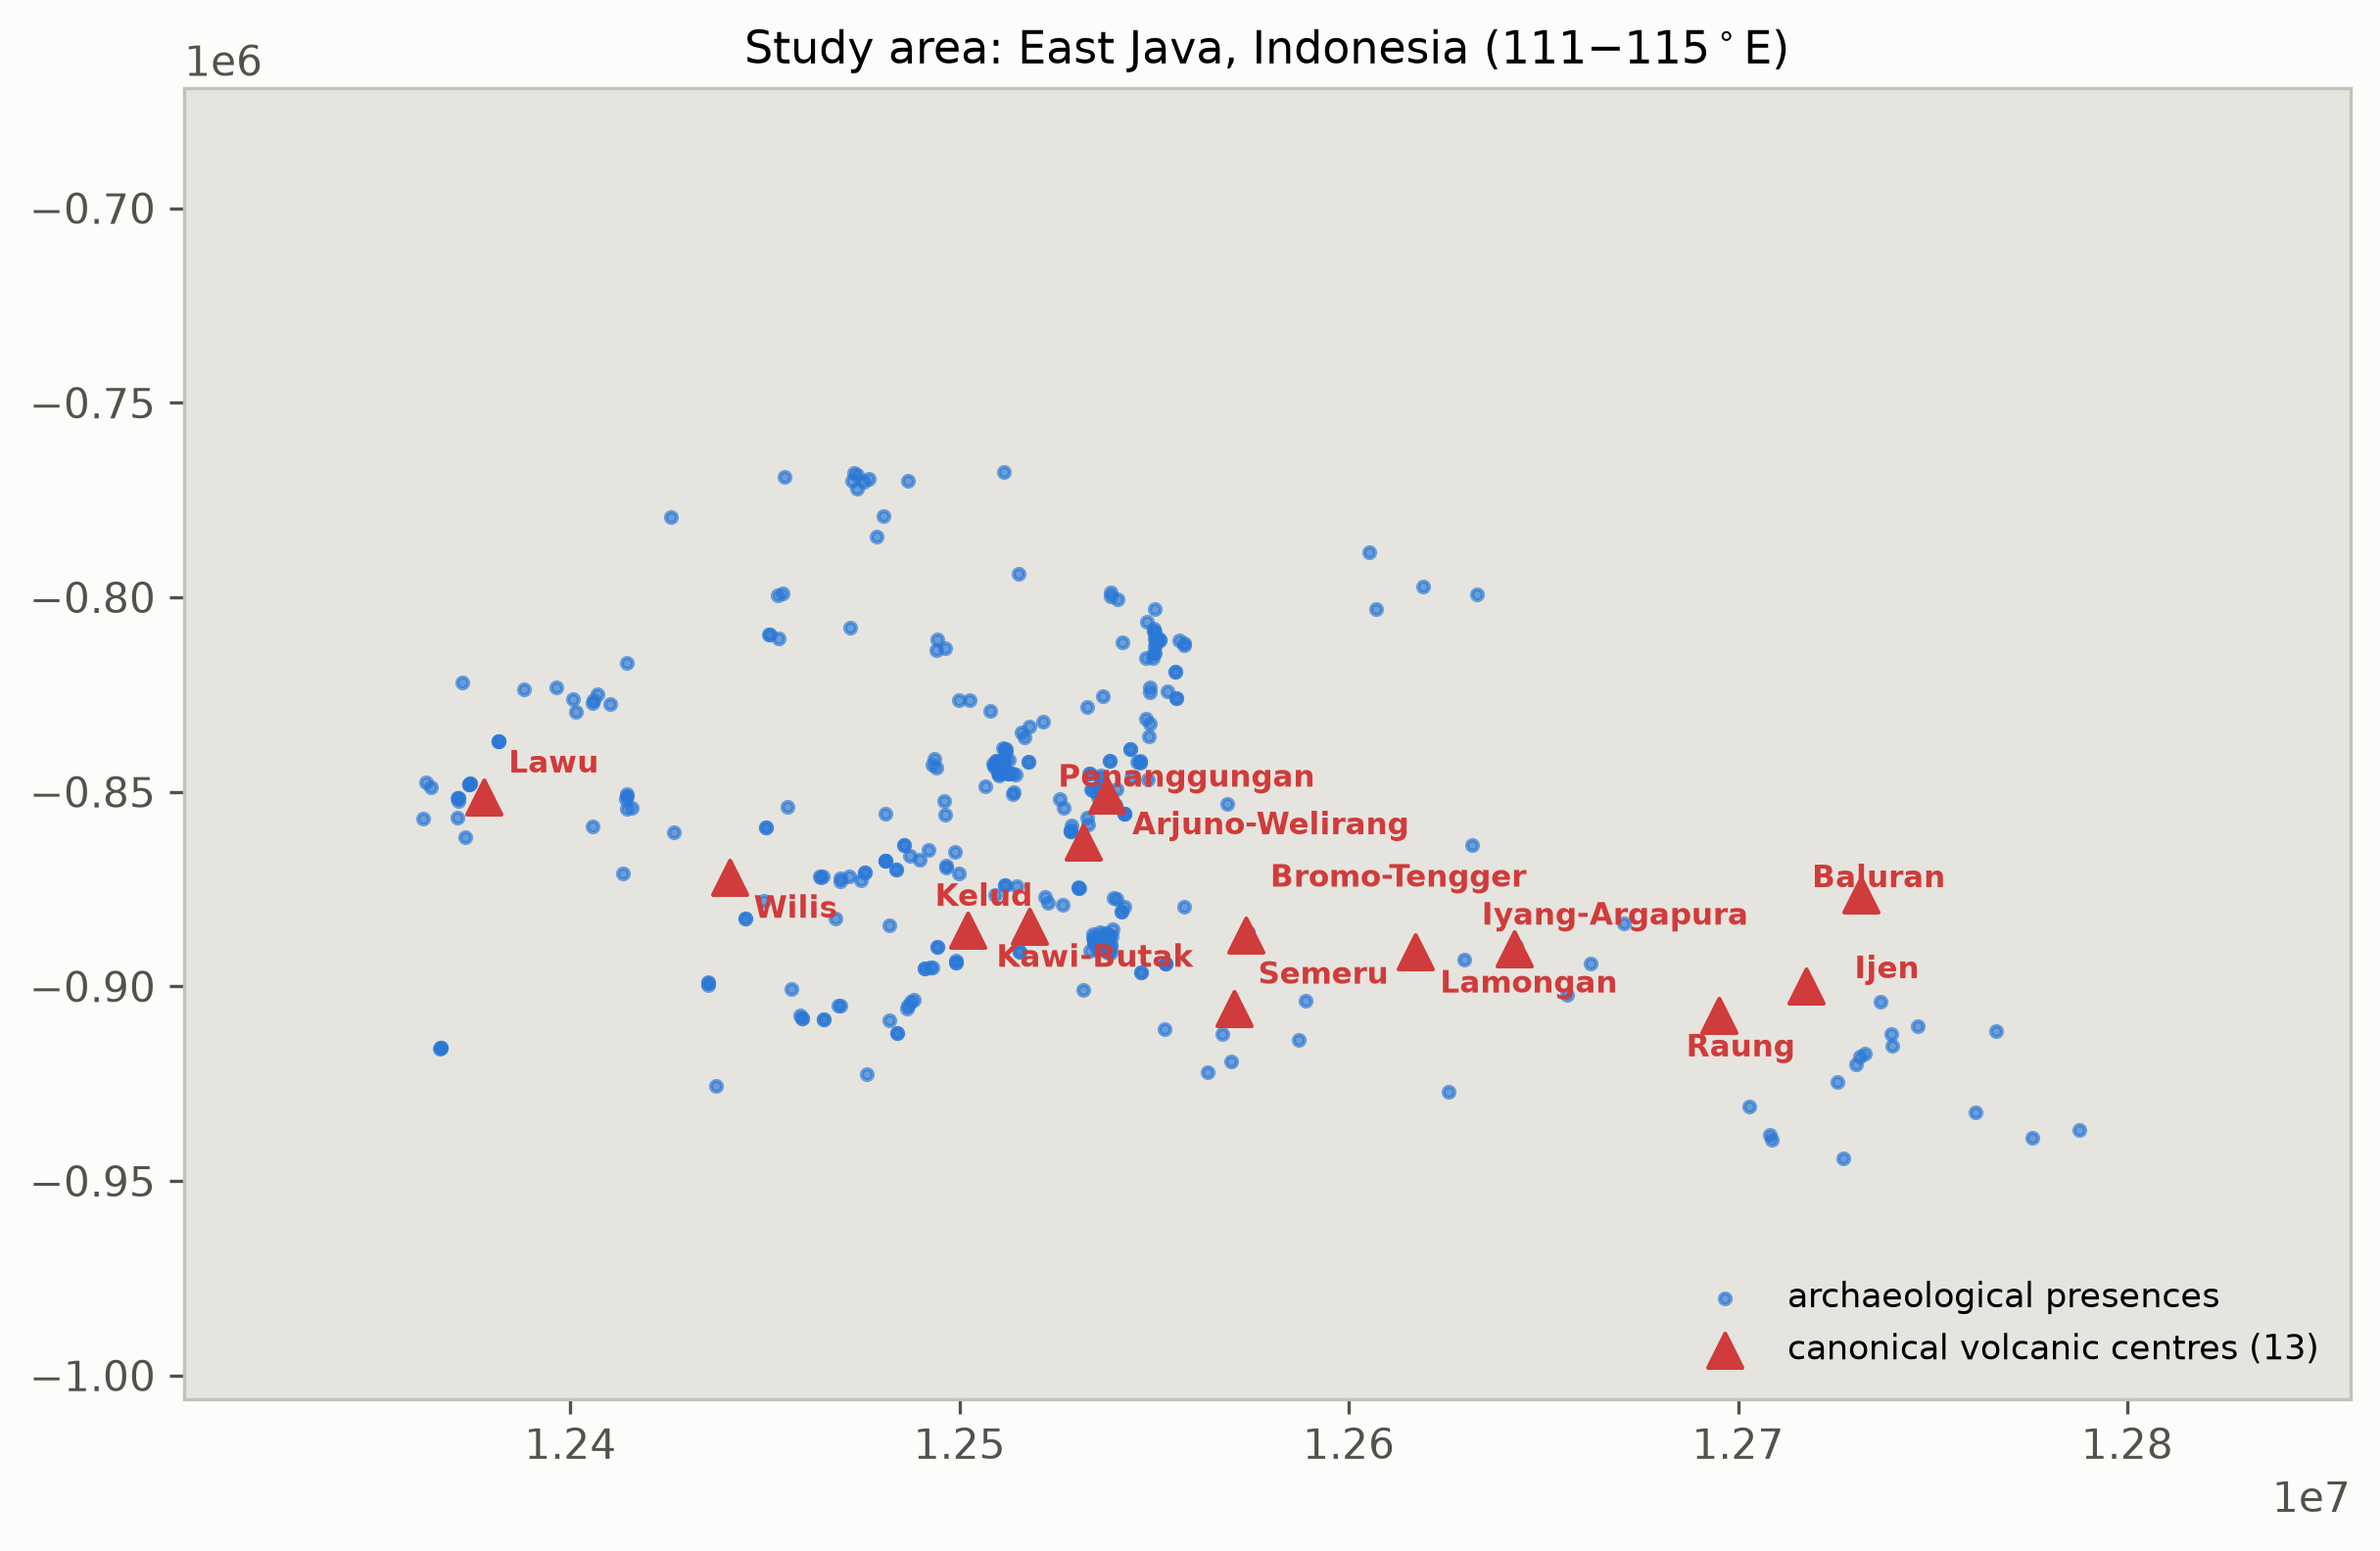
\includegraphics[width=0.9\textwidth]{fig10_study_area_map.png}
\caption{Study area in East Java, Indonesia, showing archaeological presences and the canonical volcanic centres used as post-hoc diagnostics only. [FIGURE: redraw under block E to label the canonical 13 centres inside 111--115$^\circ$E, not the legacy 7 --- see INT-1.]}
\label{fig:studyarea}
\end{figure}

% ============================================================================
\section{Materials and Methods}
% ============================================================================

\subsection{Data, covariates, and the principle of role separation}
\label{sec:covariates}

Usable presences after covariate filtering were 378 (111--115$^\circ$E); the soil-coverage subset used once in E009 was 259.
Every variable plays one analytical role, and the roles must not be mixed, because mixing them makes a suitability score uninterpretable: a low score could mean the place was unsuitable, or unsurveyed, or not preserved, and the model cannot say which.
We therefore keep only the suitability block as predictors, express accessibility through the background design (\S\ref{sec:fourroles}), and treat preservation and volcanic proximity as diagnostics applied to the output.
Table~\ref{tab:roles} assigns every variable a single role.

\begin{table}[h]
\centering
\small
\begin{tabular}{llp{5.6cm}p{4.2cm}}
\toprule
Variable & Source & Analytical role & How it enters \\
\midrule
elevation & Copernicus GLO-30 DEM, 30 m, decimated $\times$10 ($\sim$300 m) & Suitability (terrain) & training feature \\
slope & derived from DEM & Suitability (terrain cost) & training feature \\
TWI & topographic wetness index, derived from DEM & Suitability (water availability) & training feature \\
TRI & terrain ruggedness index, derived from DEM & Suitability (terrain cost) & training feature \\
aspect & derived from DEM & Suitability (insolation/orientation) & training feature \\
river\_dist & OSM/HydroSHEDS, Euclidean distance & Suitability (water access); added at E008 & training feature \\
clay, silt & SoilGrids topsoil & Preservation / substrate & features in \textbf{E009 only}; dropped (lowered AUC) \\
road\_dist & OSM roads (expanded class set from E012) & Accessibility / survey effort & \textbf{never a training feature} \\
volcano\_dist & canonical inventory, 30 centres (13 in bounds) & Taphonomy / burial --- diagnostic only & \textbf{never a training feature} \\
\bottomrule
\end{tabular}
\caption{Table 1. Covariates and their analytical roles. Roles are exclusive by construction: a suitability variable answers \emph{would people have settled here?}; an accessibility variable answers \emph{would we have found it?}; a preservation variable answers \emph{would it still be there to find?}. TWI (topographic wetness index) quantifies the tendency of a cell to accumulate water; TRI (terrain ruggedness index) quantifies local elevation difference as a proxy for terrain cost.}
\label{tab:roles}
\end{table}

This separation is not a technicality.
After the benchmark reported in \S3, it is the paper's actual subject, because the variable that defines the background (accessibility, via \texttt{road\_dist}) is the variable that turned out to drive the reported number.

\subsection{The modelling pipeline}
\label{sec:pipeline}

We model binary presence/background suitability.
The pseudo-absence (background) ratio is fixed at 1:5 throughout.
Three learners are compared: XGBoost \citep{chen2016} (primary), RandomForest \citep{breiman2001}, and a maxnet-equivalent Maximum Entropy model \citep{elith2006, phillips2006} added in response to R1-D.
Validation uses 5-fold deterministic spatial block cross-validation at a baseline block size of 0.45\textdegree{} ($\sim$50~km).
Primary metrics are AUC and the True Skill Statistic (TSS), the latter preferred to kappa for presence--background models as it is independent of prevalence \citep{allouche2006, jimenez2020}.
Our minimum viable result (MVR) criterion is spatial AUC $> 0.75$ under block cross-validation.

\subsection{The experiment progression, as the object under examination}
\label{sec:progression}

Seven iterative experiments (E007--E013) built the model whose evaluation we now examine.
They are no longer the argument of the paper; they are the object the argument is about, so we summarise them in one table and two paragraphs and move the per-iteration detail to the supplement.
Table~\ref{tab:inclusion} states exactly which covariates each experiment used, read from the analysis scripts rather than from any earlier prose.

\begin{table}[h]
\centering
\small
\begin{tabular}{lccccccccl}
\toprule
Exp. & elev & slope & twi & tri & aspect & river & road & Background design & Rep.\ spatial AUC \\
\midrule
E007 v1  & \cmark & \cmark & \cmark & \cmark & \cmark & --    & --    & uniform random, 1:5, 2 km buffer & 0.659 \\
E008 v2  & \cmark & \cmark & \cmark & \cmark & \cmark & \cmark & --    & uniform random, 1:5 & 0.695 \\
E009 v3  & \cmark & \cmark & \cmark & \cmark & \cmark & \cmark & --    & uniform random, 1:5 (+clay/silt) & 0.664 $\downarrow$ \\
E010 v4  & \cmark & \cmark & \cmark & \cmark & \cmark & \cmark & bg    & TGB (major road) & 0.711 \\
E011 v5  & \cmark & \cmark & \cmark & \cmark & \cmark & \cmark & bg    & TGB, parameters swept & 0.725 \\
E012 v6  & \cmark & \cmark & \cmark & \cmark & \cmark & \cmark & bg    & TGB, expanded road classes & 0.730 \\
E013 v7  & \cmark & \cmark & \cmark & \cmark & \cmark & \cmark & bg    & hybrid = TGB pool + regional blend + hard negatives & 0.768 best / 0.751 seed-avg \\
\bottomrule
\end{tabular}
\caption{Table 2. Per-experiment covariate inclusion. \cmark\ = training feature; -- = not used; \emph{bg} = used to construct the background, never as a feature. Reproducibility: rasters in \texttt{data/processed/dem/}, presences in \texttt{data/processed/east\_java\_sites.geojson} (378 valid in bounds), deterministic 5-fold spatial blocking at 0.45\textdegree{}, pseudo-absence ratio 1:5 throughout. E010--E013 use \texttt{road\_dist} to build the background while excluding it from the features.}
\label{tab:inclusion}
\end{table}

Two paragraphs of interpretation.
Feature-only expansion plateaued (E007--E009): adding river distance helped ($+0.036$) and adding soil covariates hurt ($-0.031$).
Background redesign then delivered the monotone rise (E010--E013) that we originally reported as evidence that pseudo-absence realism dominates feature accumulation.
The remainder of this paper asks whether that rise is real.

The hybrid design of E013 blends a TGB candidate pool with a regional quota and a fraction of ``hard negatives'' (cells environmentally dissimilar from presences, $2.0 \leq z \leq 5.0$), sweeping \texttt{region\_blend} $\in \{0.0,0.3,0.5,0.7\}$ and \texttt{hard\_frac} $\in \{0.0,0.15,0.30\}$.
Note that the realised proportion of environmentally dissimilar pseudo-absences in the best configuration was $0.62$, above the $0.30$ target: the TGB pool, constrained to road-accessible cells, is intrinsically more dissimilar from site environments than unconstrained random sampling.
This pool-composition effect bears on the absolute AUC values and is part of why a common evaluation background matters (\S\ref{sec:artefact}).

\subsection{The four roles of \texttt{road\_dist}}
\label{sec:fourroles}

\texttt{road\_dist} is deliberately never a training feature, yet it does four jobs at once: it (i) defines the TGB acceptance probability, (ii) defines the hybrid background pool, (iii) defines the accessibility-proxy holdout split (E014, \S\ref{sec:holdout}), and (iv) is a tautology proxy in Tests 1 and 3.
The submitted manuscript acknowledged this coupling once, in the limitations.
Given the benchmark in \S3, that placement was wrong: the variable that builds the background is the variable that drives the reported number, and it now appears here, where the covariates are introduced.
This is also the honest answer to the question of what makes the approach specifically archaeological: the archaeological content is not in the label set, it is in the background design --- a claim about where a survey could plausibly have detected a site had one been present.

\subsection{The accessibility-proxy holdout (E014)}
\label{sec:holdout}

E014 trains on easy-access presences (\texttt{road\_dist} $\leq 1$~km) and tests on hard-access presences ($>1$~km), using road accessibility as a proxy for discovery order: sites far from roads stand in for sites found late.
We previously called this a ``temporal split''; we now call it an \emph{accessibility-proxy holdout}, because the split is defined by access, not by date, and the earlier label overstated what the data support.
(The stored result file had itself been mislabelled with temporal headers; the underlying split is the accessibility split described here, AUC $= 0.755$ is unaffected, and the file now records which branch ran --- see the Further Disclosures in the Response to Reviewers.)

\subsection{The refutation design: E217--E224}
\label{sec:refutation}

The seven experiments that overturn the ladder were pre-registered (decision rules written before the runs) and are the paper's centrepiece.

\paragraph{E217 -- common-background benchmark (answers R1-D).}
MaxEnt, XGBoost and RandomForest are run under \emph{identical} spatial-block folds and \emph{identical} background designs as E007--E013, but each design is scored against a \emph{common} evaluation background shared across designs, so that the comparison is identified.
A second feature set (\texttt{terrain} alone, 5 vars vs \texttt{terrain\_river}, 6 vars) lets us compare a feature effect against a background-design effect.

\paragraph{E218 -- the evaluation artefact, isolated.}
Three training designs are each scored against four evaluation backgrounds (own + three foreign), exposing how much of each design's apparent lead comes from being judged at home.

\paragraph{E220 -- does the selection criterion have an interior optimum?}
We sweep the hard-negative dial and ask whether the AUC-on-own-background criterion ever tells a researcher to stop short of the dial's edge.

\paragraph{E221 -- seed stability of the priority map.}
Across random seeds, how much of the top-decile priority map turns over, and how many seeds must be ensembled to stabilise it?

\paragraph{E222 -- synthetic ground truth.}
Four synthetic worlds of known intensity surface let us compare \emph{reported} AUC (own-background) against \emph{true} recovery (common-background) where ground truth is not in question.

\paragraph{E223 -- confidence intervals and regularisation.}
Bootstrap and equivalence CIs bound the ladder gain; a MaxEnt regularisation sweep ($\beta = 0.5$--$4.0$) tests whether the artefact is an overfit of an unregularised model.

\paragraph{E224 -- a diagnostic we pre-registered and then withdrew (see \S\ref{sec:tgbnull}).}
We proposed that the TGB null in E222 was structural, tested it, and the test failed; the null is reported as unexplained.

% ============================================================================
\section{Results}
% ============================================================================

\subsection{The reported ladder}
\label{sec:ladder}

Reproducing the claim under examination: Table~\ref{tab:progression} and Figure~\ref{fig:progression} show the rise from E007 (0.659) to E013 (seed-averaged 0.751; best run 0.768; TSS $0.507 \pm 0.167$), with 20-seed stability in the range 0.729--0.774.
Even the worst seed exceeded a spatial-interpolation null (DKNS, 0.646) by $+0.083$, and the model beat the three null models in Table~\ref{tab:nullmodel}.
This is the performance we reported, and on its face it supports the conclusion we drew.

\begin{table}[h]
\centering
\resizebox{\textwidth}{!}{%
\begin{tabular}{llccccccc}
\toprule
Exp. & Pseudo-absence strategy & XGB AUC & RF AUC & Best AUC & XGB TSS & RF TSS & Status \\
\midrule
E007 & Random                 & 0.659 $\pm$ 0.077 & 0.656 $\pm$ 0.090 & 0.659 & 0.318 $\pm$ 0.126 & 0.314 $\pm$ 0.133 & REVISIT \\
E008 & Random + river feature & 0.685 $\pm$ 0.074 & 0.695 $\pm$ 0.107 & 0.695 & 0.345 $\pm$ 0.135 & 0.379 $\pm$ 0.200 & REVISIT \\
E009 & Random + soil features & 0.664 $\pm$ 0.049 & 0.643 $\pm$ 0.054 & 0.664 & 0.337 $\pm$ 0.083 & 0.312 $\pm$ 0.072 & REVISIT \\
E010 & TGB (major road)       & 0.711 $\pm$ 0.085 & 0.699 $\pm$ 0.081 & 0.711 & 0.384 $\pm$ 0.150 & 0.380 $\pm$ 0.130 & REVISIT \\
E011 & TGB tuned              & 0.725 $\pm$ 0.084 & 0.716 $\pm$ 0.081 & 0.725 & 0.447 $\pm$ 0.184 & 0.408 $\pm$ 0.147 & REVISIT \\
E012 & TGB tuned (expanded)   & 0.730 $\pm$ 0.085 & 0.724 $\pm$ 0.081 & 0.730 & 0.420 $\pm$ 0.170 & 0.413 $\pm$ 0.152 & REVISIT \\
E013 & Hybrid bias-corrected  & 0.768 $\pm$ 0.069 & 0.742 $\pm$ 0.070 & 0.768 & 0.507 $\pm$ 0.167 & 0.458 $\pm$ 0.126 & SUCCESS \\
\bottomrule
\end{tabular}}
\caption{Table 3. Experiment progression E007--E013 (the ladder under examination).}
\label{tab:progression}
\end{table}

\begin{figure}[h]
\centering
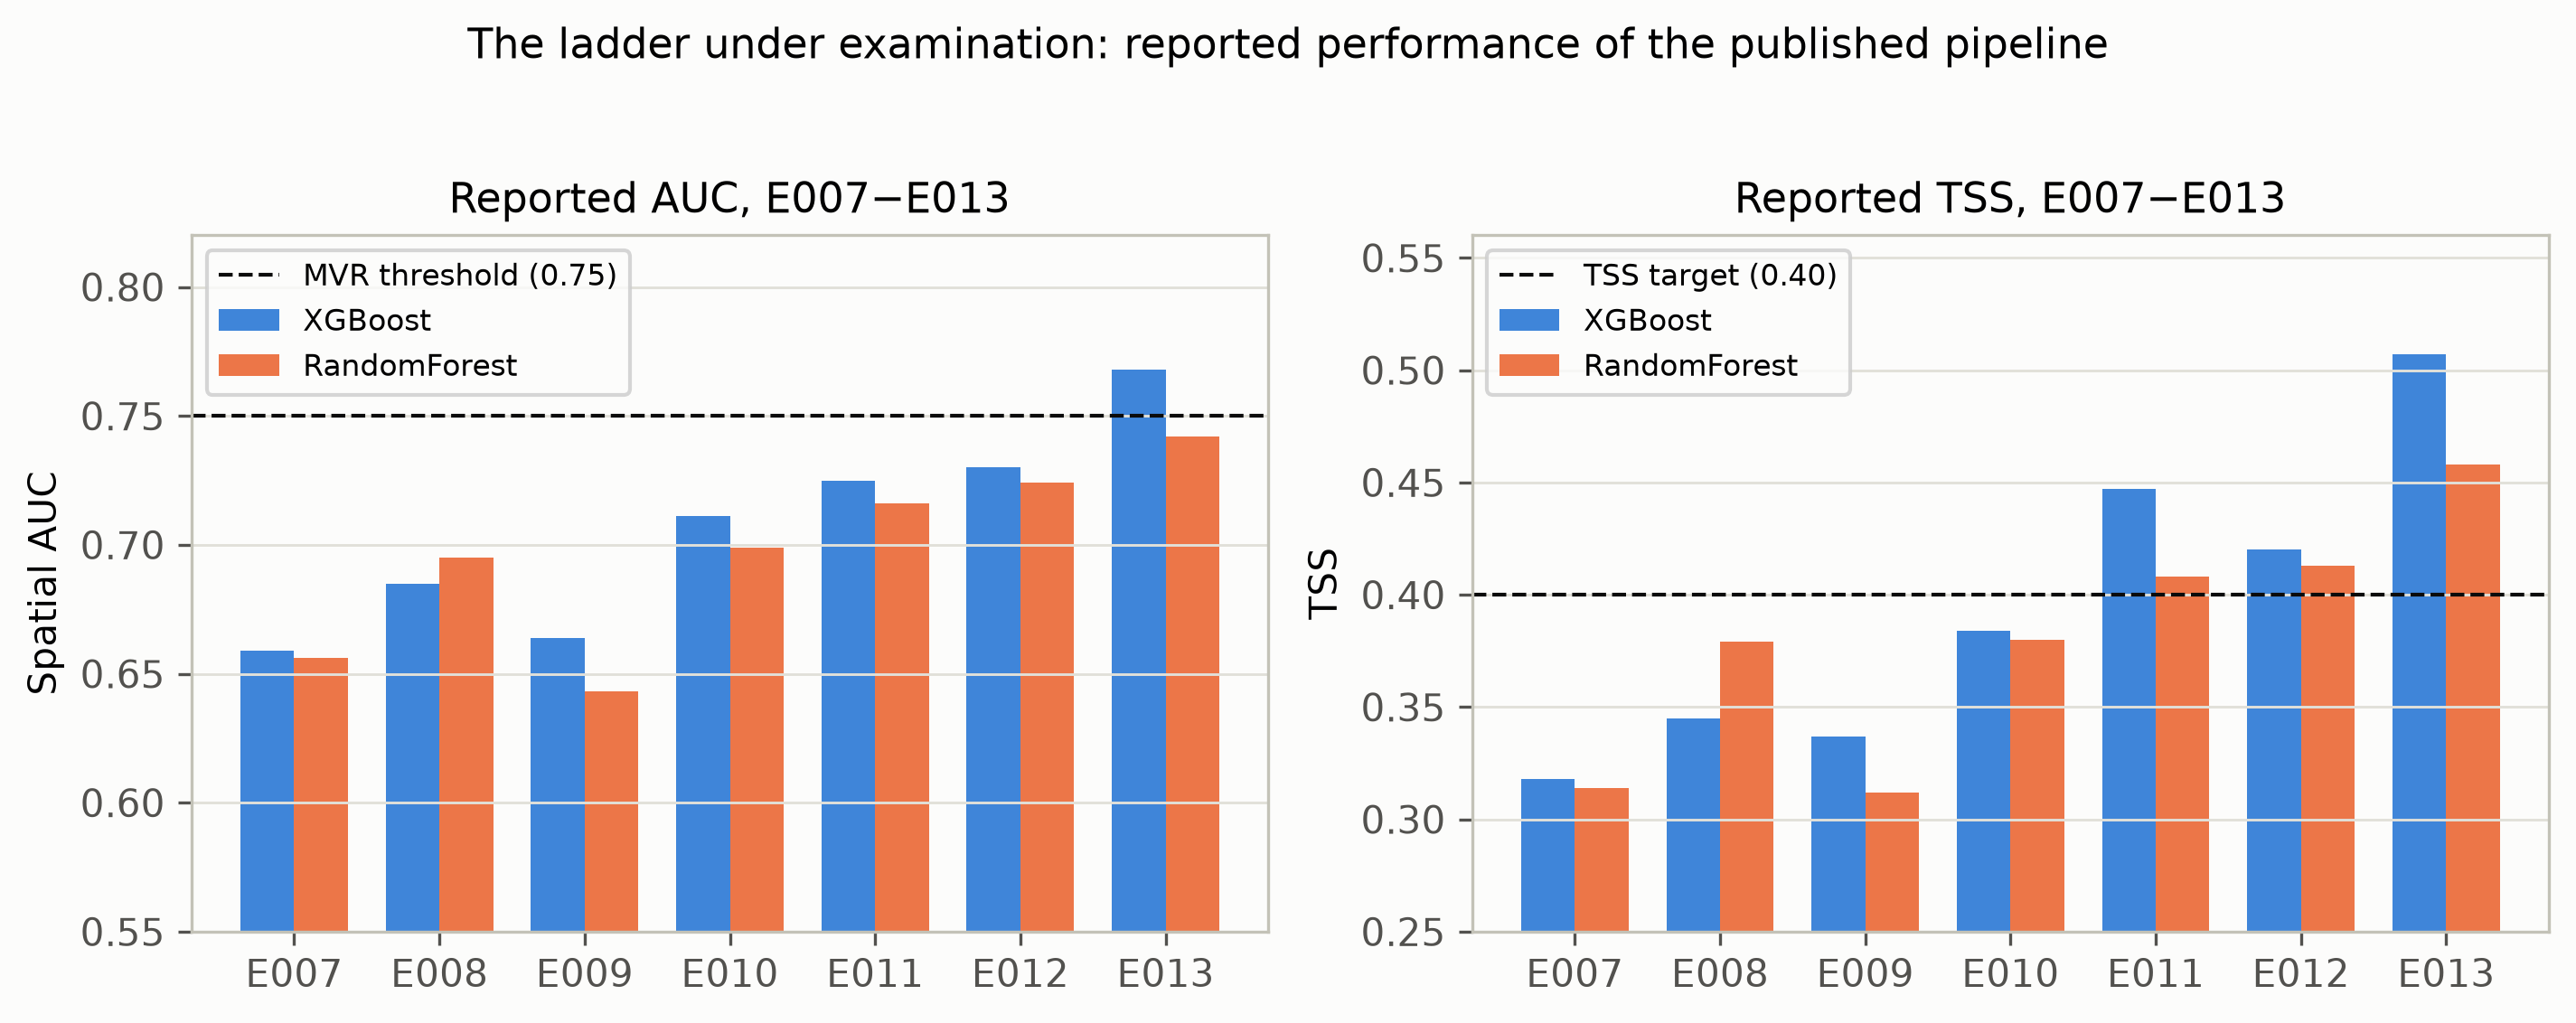
\includegraphics[width=0.95\textwidth]{fig3_auc_tss_progression.png}
\caption{AUC/TSS progression E007--E013. [FIGURE: under block E, overlay the common-evaluation-background values so the artefact is visible against the ladder in one panel.]}
\label{fig:progression}
\end{figure}

\begin{table}[h]
\centering
\small
\begin{tabular}{lccc}
\toprule
Model & AUC & Std & Gap vs E013 \\
\midrule
Random (chance)              & 0.500 & 0.000 & $+$0.268 \\
Heuristic (river $<$ 2 km)   & 0.581 & 0.054 & $+$0.187 \\
DKNS (spatial interpolation) & 0.646 & 0.032 & $+$0.122 \\
\textbf{E013 XGB (seed-avg)} & \textbf{0.751} & 0.013 & --- \\
E013 XGB (best run)          & 0.768 & 0.069 & --- \\
\bottomrule
\end{tabular}
\caption{Null-model comparison under spatial CV. DKNS (distance to known nearest site) uses site locations as an unfair upper bound; E013 exceeds it by $+$0.122 with environmental features only. The ladder exceeds these nulls; \S\ref{sec:artefact} asks whether the rise \emph{between} E007 and E013 is real.}
\label{tab:nullmodel}
\end{table}

\subsection{The ladder is an evaluation artefact}
\label{sec:artefact}

It is not.
On real data, redesigning the background while holding a common evaluation background fixed contributes \textbf{$-0.0142$ AUC} averaged over the three algorithms, whereas adding the river feature contributes \textbf{$+0.0424$ AUC}, positive in 12/12 paired comparisons (the redesign contribution is $+0.0054$ on the terrain-only feature set and $-0.0142$ on the full set; we state the feature set so a reader does not encounter the difference unannounced).
The hybrid design beats the random design in 3/3 algorithms when each is scored on the \emph{hybrid} evaluation background, and in \textbf{0/3} on each of the uniform, target-group and stratified evaluation backgrounds.
The advantage evaporates the moment it is judged anywhere but at home.

How large is judging at home?
The inflation from own-background evaluation is positive in \textbf{60/60} seed$\times$algorithm cells (mean $+0.037$, range $+0.005 \ldots +0.084$) --- the same order of magnitude as the entire reported E007$\rightarrow$E013 gain.
Aggregated over the synthetic worlds, a model scored on its own background is reported higher than its truth in \textbf{343/360 runs (95.3\%; median $+0.187$, minimum $-0.031$)}.
We reject the published ladder gain ($+0.092$) directly: equivalence confidence intervals exclude it in \textbf{12/12} algorithm$\times$evaluation-background cells, and a spatially blocked bootstrap rejects it for all three algorithms (CI upper bounds $+0.008$, $+0.025$, $+0.026$).
Changing the MaxEnt regularisation $\beta$ across $0.5$--$4.0$ changes nothing ($-0.020$ to $-0.022$, 1/10 runs positive), so the artefact is not an overfit of an unregularised model.

\begin{figure}[h]
\centering
\figtodo{Two-panel: (left) reported AUC vs common-background AUC across the E007--E013 designs, three algorithms; (right) histogram of own-background inflation across 360 synthetic runs, with the $+0.092$ published gain marked. Source: e218\_stageA\_raw.csv, e222\_runs.csv, e223a/b.}
\caption{Figure 4. The evaluation artefact. Left: the ladder flattens or reverses under a common evaluation background. Right: own-background inflation is positive in 95.3\% of synthetic runs.}
\label{fig:artefact}
\end{figure}

\subsection{The selection criterion has no interior optimum}
\label{sec:nooptimum}

Why does the ladder exist at all?
The selection criterion --- AUC computed on a design's own background --- has no interior optimum: its maximum always sits at the edge of whatever dial is swept.
In the synthetic worlds the criterion rises monotonically along the hard-negative dial ($0.7367 \rightarrow 0.8904$); on the real data it is monotone from $0.1$ upward, with one dip of $-0.0071$ at $0.0 \rightarrow 0.1$.
Because the criterion never points inward, it never tells a researcher to stop.

The practical consequence is mild at the operating point our manuscript used.
We stopped at \texttt{hard\_frac} $= 0.30$ because our grid stopped there, not because the criterion said to; the cost of that stop, against the truth-best configuration on the same grid, is small ($+0.0044$ real; median $+0.0000$ synthetic, mean $+0.0012$, maximum $+0.0088$), and on the manuscript's own grid the criterion does not pick the truth-best design in 29/60 cases but the differences are essentially zero.
The danger is structural: if the dial were extended, the cost is large ($+0.0973$ real; $+0.1937$ synthetic median, $100\%$ positive), and the criterion provides no brake.
We note what the criterion does \emph{not} do, correcting an earlier internal claim: the design it selects (hybrid(1.0)) is never the truth-worst design; the truth-worst is hybrid(0.0) in 50/60 cases. The selected design costs \textbf{$+0.194$ AUC$_{\text{true}}$ against the best available}, but it is not the worst.

\begin{figure}[h]
\centering
\figtodo{Dose-response: reported (own-background) and true (common-background) AUC against the hard\_frac dial, synthetic and real, three algorithms. Mark the manuscript's stop at 0.30 and the grid edge. Source: e218b\_hardfrac\_sweep.csv, e222\_runs.csv.}
\caption{Figure 5. The selection criterion on a design's own background (solid) keeps rising to the edge of the dial; the true performance (dashed) does not. The criterion has no interior optimum.}
\label{fig:dial}
\end{figure}

\subsection{Reported and true performance diverge}
\label{sec:diverge}

In the synthetic worlds the reported number moves about \textbf{twice} as fast as the truth along the dial ($+0.1538$ reported vs $+0.0764$ truth; endpoint ratio $2.01\times$, per-run OLS slope $2.12\times$, per-run median ratio $2.00\times$ --- we name the estimator because the three definitions bracket ``about twice'').
On the real data the two move in \textbf{opposite directions} ($+0.1227$ reported vs $-0.0973$ common-background), which is a stronger statement and needs no magnification.
A pre-registered prediction that own-background inflation rises with the hard-negative fraction in every regime \textbf{failed} (pooled Spearman $0.4395 < 0.5$) and is reported as failed.

\subsection{The target-group-background null, reported as unexplained}
\label{sec:tgbnull}

Our synthetic worlds gave TGB exactly the condition its theory requires --- a known, survey-biased observation process --- and TGB did not help.
Over the synthetic runs, TGB minus random on top-decile map agreement (Jaccard) is $-0.010$, positive in $46.7\%$ of paired comparisons.
In regional-bias regimes TGB is neutral rather than harmful (World C $-0.0010$, $56.7\%$ positive; World D $+0.0022$, $73.3\%$ positive), and it wins only under model misspecification (Jaccard $0.4504$ vs $0.4458$ in World B), which we report because it is true but do not build on.

We proposed an explanation for this uncomfortable null and nearly wrote it into the manuscript: because \texttt{road\_dist} is not a model feature, the survey-bias factor is unrepresentable in feature space, so TGB has nothing to cancel --- a tidy, ``predicted'' null.
We pre-registered a test with both decision branches written first, then ran it (E224): the same synthetic worlds with \texttt{road\_dist} added to the features.
It made no difference.
TGB minus random was $-0.0217$ with \texttt{road\_dist} in the features (30\% positive) and $-0.0254$ without (30\% positive).
We therefore report the null as \textbf{unexplained}, and we disclose the limitation of our own test: \texttt{road\_dist} correlates $+0.49$ with \texttt{river\_dist} (and $+0.31$ with elevation), so the model already had partial access to the bias signal in the control condition; a clean test needs a survey-effort surface orthogonal to terrain by construction, which is future work.
We resisted re-interpreting the secondary metric (\texttt{auc\_true}, which did rise from $36.7\%$ to $60\%$ positive) because the pre-registered primary metric was map Jaccard, and map Jaccard said no.

\subsection{Confidence intervals and a detection floor}
\label{sec:ci}

The equivalence CIs that reject the $+0.092$ gain (\S\ref{sec:artefact}) also bound what we can rule out: at $n=378$ the spatially blocked bootstrap cannot exclude effects below about $+0.03$.
Findings smaller than that are indeterminate at this sample size, not absent.

\subsection{Priority maps are unstable under seed, and the protocol that fixes them}
\label{sec:prioritymaps}

A model whose numbers are artefactual still produces a priority map, and in heritage practice the map is what gets used.
Across random seeds, $28.1\%$--$47.4\%$ of top-decile cells turn over between seed pairs --- a single-seed map is not a defensible basis for a survey decision.
The remedy is cheap and we now make it a protocol: seed-ensemble.
The number of seeds required to stabilise the map is $k^* = 2$--$5$ for Jaccard $\geq 0.85$, \textbf{$4$--$7$ for $\geq 0.90$}, and $7$--$9$ for $\geq 0.95$; we recommend $k \geq 7$.
The ensemble admits a useful product: a \emph{robust core} (cells selected by every seed) and a \emph{contingent fringe}.
Observed site density in the robust core is higher than in the fringe by \textbf{$1.93\times / 4.34\times / 5.62\times$} for RandomForest / XGBoost / MaxEnt (we give all three rather than a rounded range, because the lower bound is $1.9$, not $2$).
We present this as \emph{consistency}, not validation: the non-volcanic comparator arm contains only $n=2$ known sites.

\subsection{Corrected tautology diagnostics, and a number that does not reproduce}
\label{sec:diagnostics}

Three corrections to our own diagnostics, none prompted by the reviewers.

\textbf{The volcano inventory.} The analysis code hard-coded 7 volcanic centres; the canonical inventory contains \textbf{13} inside the paper's own 111--115$^\circ$E bounds (adding Lawu, Wilis, Kawi-Butak, Penanggungan, Iyang-Argapura, Baluran), and two of the additions sit inside the Malang--Mojokerto site concentration.
\texttt{volcano\_dist} is not a training feature, so model AUCs are unaffected; the Test 1 tautology diagnostic is.
Recomputed on the canonical inventory, the suitability--volcano-distance Spearman correlation is $\rho = -0.281$ (legacy 7-volcano re-run: $-0.243$).
The verdict is unchanged: $|\rho| < 0.5$, so the test still passes.

\textbf{A published number that does not reproduce.} The submitted manuscript reported $\rho = -0.163$ for that same correlation, taken from a single model instance.
A five-seed re-run on the same 7-volcano inventory gives \textbf{$-0.243$}.
This is the seed instability of \S\ref{sec:prioritymaps} appearing \emph{inside} the manuscript's own tautology diagnostic, and it is direct internal evidence that the seed-ensemble protocol is needed, not optional.
Every value in this revision is seed-ensembled.

\textbf{The terrain-matched control.} A reviewer asked whether low suitability near volcanoes reflects burial or merely rugged terrain (R2-F).
We coarsened-exact-matched raster cells on elevation $\times$ slope $\times$ TRI $\times$ TWI (90 strata), comparing volcanic uplands with East Java's non-volcanic uplands (Southern Mountains karst, Kendeng limestone).
Matched mean suitability is $0.2249$ (volcanic) vs $0.1702$ (non-volcanic) and site density is $0.01377$ vs $0.00048$ sites/km$^2$ --- directionally consistent with a volcanic-specific effect, but with $n=2$ in the non-volcanic arm it is consistency, not validation.

\subsection{The taphonomic claim is withdrawn, and a quota design that failed}
\label{sec:withdrawal}

The taphonomic interpretation we built on the ladder --- that low predicted suitability near volcanoes is evidence of buried settlement --- is withdrawn, because the model comparison that supported it does not survive the common-background benchmark (\S\ref{sec:artefact}).
Low predicted suitability near a volcano is not evidence of a buried site, in the reviewer's own terms (\S\ref{sec:taxonomy}: mechanism 3 cannot be read off a suitability surface).
We also report, without softening, a quota background design we tested in its home regime (regional survey bias) and in its most favourable regime (balanced-regional truth): it failed in both (World C: $-0.2457$ AUC$_{\text{true}}$, $-0.4688$ Jaccard, 0/30; World D: $-0.2027$ AUC$_{\text{true}}$, $-0.2826$ Jaccard, 0/30).

% ============================================================================
\section{Discussion}
% ============================================================================

\subsection{The lesson: hold the evaluation background fixed}

The central methodological finding is that a background-design comparison is not identified unless the evaluation background is held fixed across the designs being compared, and that the artefact this produces is large enough to masquerade as a result.
We are not the first to worry that background choice drives reported performance \citep{phillips2009, georganos2021}; what we contribute is the mechanism (a selection criterion with no interior optimum, \S\ref{sec:nooptimum}) and a direct quantification of the inflation it produces (95.3\% of synthetic runs; 60/60 real seed$\times$algorithm cells).
The practical recommendation follows directly: \emph{report background designs on a common evaluation background, and state the evaluation availability domain of every metric}.
A metric without a declared availability domain is the lesson of this line of work, learned about our own model.

\subsection{The archaeological content is in the background}

What makes a presence--background model archaeological, rather than a generic classifier run on coordinates, is not the label set.
It is the background design: a statement about where a survey could plausibly have detected a site had one been present.
That is what TGB and hybrid designs encode, and it is why they are archaeological choices rather than sampling conveniences.
The sharp corollary, which this paper exists to state, is that because the archaeological content lives in the background, and because the model was evaluated against that same background, the very thing that made the design archaeological is what contaminated its evaluation.

\subsection{A suitability surface is not a discovery map}

With the site-prediction claim withdrawn, the output is a suitability surface with declared limits, not a map of where sites are.
Low suitability does not mean ``buried'' or ``destroyed''; high suitability does not mean ``a site is there'' (\S\ref{sec:taxonomy}).
This restraint is now stated in the manuscript in these words, and it is a constraint the revised paper takes seriously rather than a caveat appended to an overclaim.

\subsection{Implications for heritage management in East Java}

Under Indonesia's Cagar Budaya framework (UU 11/2010), BPCB Jawa Timur surveys inform permitting and rescue prioritisation.
A suitability surface could in principle support that workflow, but only under two conditions this revision makes explicit.
First, because priority maps turn over by $28$--$47\%$ between seeds (\S\ref{sec:prioritymaps}), a single-seed map is not a defensible basis for a permit; the seed-ensemble protocol ($k \geq 7$) is a precondition for operational use.
Second, because the model reports suitability and not presence, the robust core ($1.9$--$5.6\times$ the site density of the fringe) is a prioritisation aid, not a prediction: it ranks where to look, not what will be found.

\subsection{The corrected protocol}

We summarise the protocol that follows from the above, which is the constructive contribution of the revision:

\begin{enumerate}
  \item \textbf{Hold the evaluation background fixed} when comparing background designs; report own-background numbers only alongside common-background numbers.
  \item \textbf{Declare the availability domain} of every metric (background design, benchmark, selection rule).
  \item \textbf{Seed-ensemble priority maps} ($k \geq 7$); report a robust core and contingent fringe, never a single-seed map.
  \item \textbf{Treat the selection criterion as unbraked}: because it has no interior optimum, justify any stop on the design dial externally, not by the criterion's own maximum.
\end{enumerate}

\subsection{Limitations}
\label{sec:limitations}

\begin{enumerate}
  \item \textbf{Calibration gap between synthetic and real.} At the manuscript's operating point the selection criterion picks hybrid on real data but random on synthetic data, so the synthetic worlds do not reproduce the real-data selection behaviour there. This limits transferring the E222 conclusions back to the real case, and is stated here rather than hidden in a supplement.
  \item \textbf{The truth-slope sign is regime-contingent} --- negative on real data, positive on synthetic. We do not claim ``hard negatives are always bad.''
  \item \textbf{Four synthetic regimes are not a universal result.} Across the four worlds (road-bias, misspecified, regional-bias, balanced-regional-truth; $n \approx 300$--$500$), no background design beat uniform on truth. This is not a refutation of target-group background in general \citep{phillips2009}; it is a result for the regimes and sample sizes tested.
  \item \textbf{A detection floor of $\sim +0.03$} at $n=378$: smaller effects are indeterminate, not absent (\S\ref{sec:ci}).
  \item \textbf{The Boyce index is a direction check, not a selector.} Its optimum is uncalibrated to truth (median $+0.50/+0.54$, borderline); we use it only to confirm direction, and we have aligned the audit flag with this narrative so the two do not contradict.
  \item \textbf{$n=2$ in the non-volcanic arm} of the terrain-matched control: the density ratios are consistency, not validation (\S\ref{sec:diagnostics}).
  \item \textbf{The two-stage ``suitable but absent'' decomposition} (R2-C) is declared future work: it tests \emph{why} sites are absent, which requires the site-prediction claim we have withdrawn, and burial-depth data at survey resolution are not yet available.
  \item \textbf{External transfer beyond East Java is untested.}
\end{enumerate}

% ============================================================================
\section{Conclusions}
% ============================================================================

The AUC ladder we reported --- from 0.659 (E007) to 0.751/0.768 (E013), attributed to increasingly realistic pseudo-absence design --- is an evaluation artefact.
Each background design was scored against the negatives it had selected for itself; judged on a common evaluation background, redesigning the background contributes $-0.014$ AUC and adding one hydrological feature contributes $+0.042$.
The selection criterion that produced the ladder has no interior optimum, so it never tells a researcher to stop, and reported and true performance move in opposite directions on the real data.
We withdraw the taphonomic interpretation we built on the ladder, and we correct two defects in our own diagnostics (the volcano inventory and a correlation that does not reproduce across seeds).

The contribution that remains is the diagnosis and the protocol: compare background designs only on a held-fixed evaluation background, declare the availability domain of every metric, and seed-ensemble priority maps ($k \geq 7$).
We offer these not as a consolation for a lost headline but as the more useful finding the reviewer's request produced: a mechanical account of why presence--background comparisons can look decisive when they are not, and a cheap, checkable protocol that keeps the next comparison honest.
We have applied it to our own work, including to the internal revision drafts that preceded this manuscript, where the same failure mode recurred and only a blind re-derivation caught it.

% ============================================================================
\section*{Supplementary Materials}
% ============================================================================

\begin{itemize}
  \item \textbf{Table S1:} Seed stability --- XGBoost and RandomForest AUC across 20 alternate seeds for E013.
  \item \textbf{Table S2:} Block-size sensitivity --- spatial CV at $\sim$40, $\sim$50, $\sim$60 km.
  \item \textbf{Tables S3--S5:} E217 common-background benchmark; E218 own- vs common-background matrix; E222 synthetic-world reported-vs-true tables.
  \item \textbf{Table S6:} Per-experiment covariate inclusion, E217--E224 (extends Table 2).
\end{itemize}

% ============================================================================
\section*{Acknowledgements}
% ============================================================================

The authors thank the editor and two reviewers; the request to benchmark against Maximum Entropy produced the finding this paper reports.

\subsection*{Funding}
This research received no external funding.

\subsection*{Competing Interests}
The authors declare no competing interests.

\subsection*{Authors' Contributions}
M.A.\ conceived the research design, developed the methodology, implemented software, conducted formal analysis, curated data, created visualisations, and wrote the original draft.
G.F.G.\ contributed to methodology refinement, code review, and manuscript editing.
Both authors approved the withdrawal of the central claim reported in this revision.

\subsection*{Data Availability}

\textbf{Archaeological site data:} the compiled East Java site dataset is in the repository at \texttt{data/processed/east\_java\_sites.geojson} (378 with valid covariates in bounds). Sources: OpenStreetMap (ODbL), Wikidata (CC BY-SA), Wikipedia Indonesia, BPCB Jawa Timur publications.

\textbf{Environmental covariates:} Copernicus GLO-30 DEM and derived layers from the Copernicus Programme (ESA), \url{https://dataspace.copernicus.eu/}. OpenStreetMap road and river data, \url{https://openstreetmap.org} (ODbL).

\textbf{Code:} all source code, including E217--E224 and the verification script \texttt{verify\_headline\_numbers.py}, is at \url{https://github.com/neimasilk/volcarch-repo} (MIT licence). Full Python versions in \texttt{requirements\_submission\_lock.txt}.

\textbf{Interactive dashboard:} \url{https://volcarch-dashboard.streamlit.app}.

\subsection*{AI Disclosure}

AI-assisted tools (Claude, Anthropic) were used during manuscript preparation for code development, data-analysis scripting, and figure generation.
The AI tools did not contribute to research design, hypothesis formulation, or scientific interpretation.
All results were independently verified by the authors, and every headline number in this revision was re-derived blind from the raw per-run outputs before submission.

\bibliography{references}

\end{document}
